\documentclass[a4j,12pt,]{jarticle}
 \usepackage{float}
 \usepackage{siunitx} %%SI単位系用
 \usepackage{amssymb, amsmath}
 \usepackage{ascmac,here,txfonts}
 \usepackage{hyperref}
 \usepackage{listings}
 \usepackage{pxjahyper}
 \usepackage[dvipdfmx]{graphicx}
 \usepackage{amssymb, amsmath}
  \usepackage{listings}
  \usepackage[dvipdfmx]{color}
 
 \lstset{
   language={Python},
   basicstyle={\ttfamily},
   identifierstyle={\small},
   commentstyle={\small\itshape},
   keywordstyle={\small\bfseries},
   ndkeywordstyle={\small},
   stringstyle={\small\ttfamily},
   frame={single},
   breaklines=true,
   columns=[l]{fullflexible},
   numbers=left,
   xrightmargin=0zw,
   xleftmargin=3zw,
   numberstyle={\scriptsize},
   stepnumber=1,
   numbersep=1zw,
   lineskip=-0.5ex,
 }
\begin{document}

{\noindent\small 第14回報告書 \hfill\today}
\begin{center}
  {\Large 自作関数により生成した日射量データの位相差分析}
\end{center}
\begin{flushright}
  祖父江匠真 \\
\end{flushright}

\section{概要}
今回は, 自作関数で生成した日射量データと, これを複製し, 時刻データにずれ時間を加えたデータとの間の位相差を計算して, ずれ時間と位相差の関係を調査した.

\section{自作関数で生成した日射量データについて}
位相差の計算には, 自作関数で生成した図 \ref{p1} に示す日射量データを使用した.

この日射量データは, 午前6時に立ち上がり, 正午に1 \si{\kilo\watt/m^2}を通り, 午後6時に0 \si{\kilo\watt/m^2}を通るようになっている.

\begin{figure}[H]
  \begin{center}
    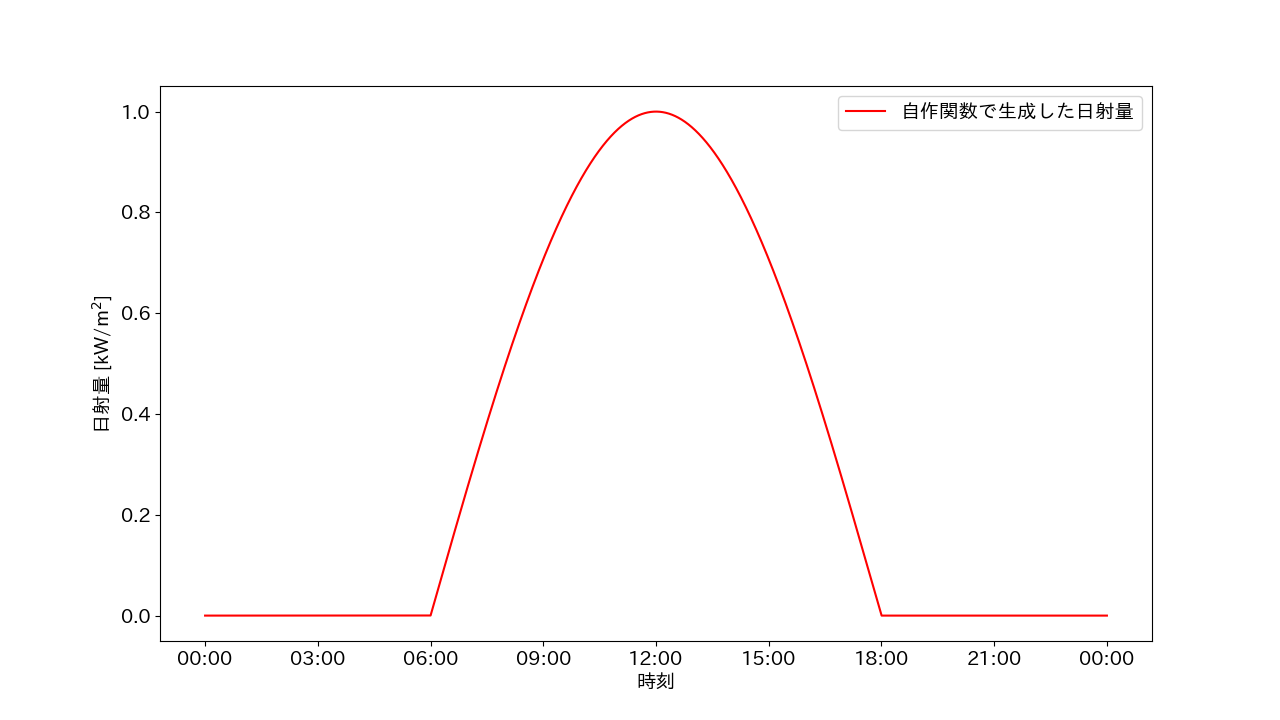
\includegraphics[width=160mm]{simulated.png}
    \caption{自作関数で生成した日射量データ}
    \label{p1}
  \end{center}
\end{figure}

\section{位相差を求める手順}

ずれ時間とその値に対応する位相差の計算は, 以下手順を繰り返し実行して行った.

\begin{enumerate}
  \item scipy.fft.fft メソッドを使用して, 自作関数で生成した日射量データと複製データの高速フーリエ変換(FFT)を行い, 振幅スペクトルを取得する.  
  \item numpy.abs メソッドを使用して, 振幅スペクトルで最も振幅が大きい周波数に対応するフーリエ係数の位相をnumpy.angleメソッドを用いて求め, 自作関数で生成した日射量データと複製データの位相差を計算する. 
  \item numpy.roll 関数を使用して複製データの時刻データを1sずつ遅らせる方向にずらす. 
\end{enumerate}

本検証では, この計算を0sから1000sまでのずれ時間で繰り返し行った. 

\section{結果}
結果として, 図 \ref{p2}に示すグラフが得られた. 横軸がずらした時間の秒数, 縦軸が位相差となっている. 図 \ref{p2}から, 自作関数で生成した日射量データを用いた場合, ずれ時間を加えていない複製データとの間の位相差は0 \si{\radian}となった.

\begin{figure}[H]
  \begin{center}
    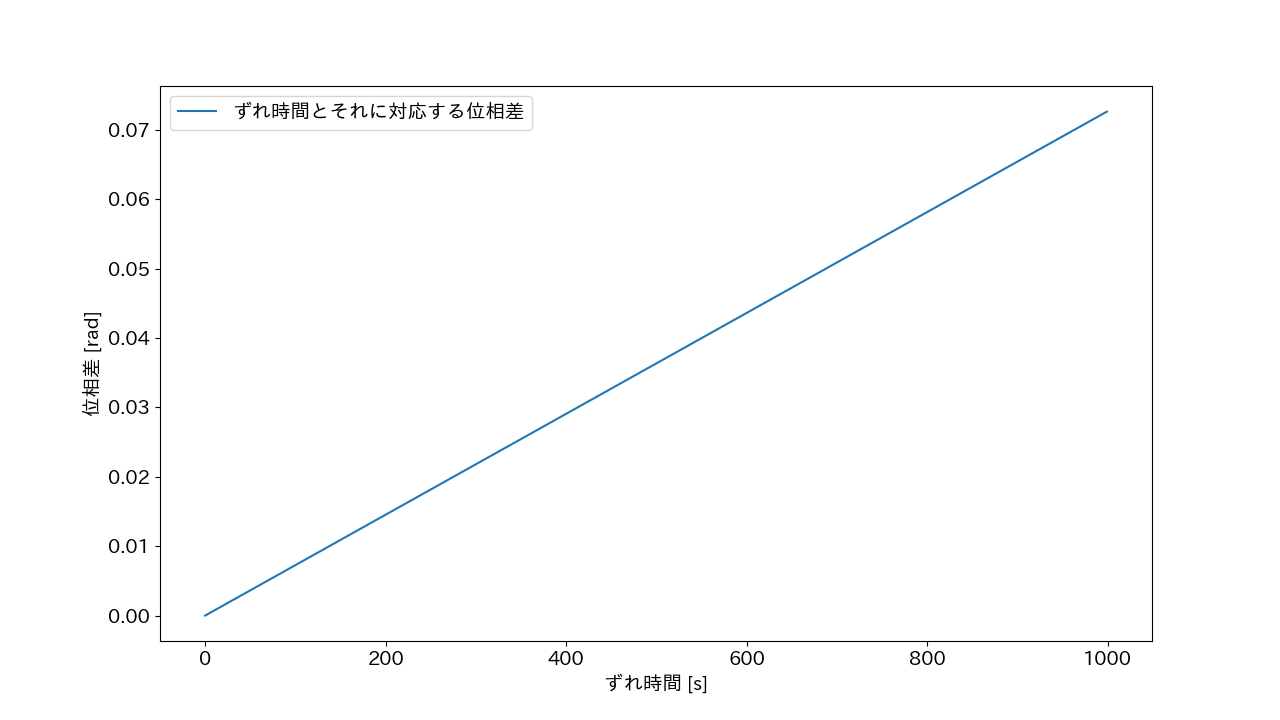
\includegraphics[width=160mm]{phase_difference.png}
    \caption{ずれ時間と位相差}
    \label{p2}
  \end{center}
\end{figure}

\section{まとめ}
今回は, 自作関数で生成した日射量データと, これを複製し, 時刻データにずれ時間を加えたデータとの間の位相差を計算して, ずれ時間と位相差の関係を調査した.

結果として, ずれ時間に対して位相差が線形的に変化し, 自作関数で生成した日射量データと, ずれ時間を加えていない複製データの位相差は0 \si{\radian}となった.

次回は, Pblivによって得られたシミュレーションデータ同士で位相差の計算を行い, ずれ時間を加えていない条件における位相差が0 \si{\radian}になるか検証する.
\end{document}